\documentclass{article}

\usepackage{fullpage}
\usepackage{url}
\usepackage{graphicx}
\usepackage{amsmath}
\usepackage{amssymb}
\usepackage{amsthm}
\usepackage{physics}
\usepackage{mathtools}

\DeclareMathOperator{\erfi}{erfi}
\newcommand{\R}{\ensuremath{\mathbb{R}}}

\title{Quantum Mechanics I Excercise 4}
\author{Idan Stark}
\date{\today}

\begin{document}
\maketitle

\section{Landau levels in a well}
In this section we will discuss the effects on the eigenstates of a particle in a magnetic field when a well is added.
Classically, the motion of a particle with charge $q$ in a uniform magnetic field $\boldsymbol{B} = B\hat{z}$ is:
\begin{equation}
    v_z = const \qquad v_x = v\cos(\omega_c t + \alpha) \qquad v_y = v\sin(\omega_c t + \alpha)
\end{equation}
\begin{equation}
    z(t) = v_z t \qquad x = x_0 + \frac{v}{\omega_c}\sin(\omega_c t + \alpha) \qquad y = y_0 - \frac{v}{\omega_c}\cos(\omega_c t + \alpha)
\end{equation}
where
\begin{equation}
    x_0 = x - \frac{v_y}{\omega_c} \qquad y_0 = y + \frac{v_x}{\omega_c}
\end{equation}
are the center of the circular motion in the x-y plane and are constants of motion, together with $v$ which is determined by the energy, and
\begin{equation}
    \omega_c = \frac{qB}{m}
\end{equation}
is the cyclotron frequency. The radius of the circular motion in x-y plane is then
\begin{equation}
    r_{c} = \frac{v}{\omega_c} = \frac{mv}{qB}
\end{equation}
\subsection{The classical case, one wall}
In the classical case, adding a wall at $x = a$, i.e. adding the effective potential
\begin{equation}
    U(x) = \begin{cases} 0 & x < a \\ \infty & x \ge a \end{cases}
\end{equation}
prevents solutions in a certain region of space to occour. Since classically it takes infinite energy to traverse the wall, any trajectory that passes even partially through it, is no longer a solution, while the rest of the space remains unchanged. This gives a boundary to constant $x_0$:
\begin{equation}
    x_0 < a - r_c
\end{equation}
for which the trajectory is unaffected. On the other side, trajectories with $x_0 > a + r_c$ are completely beyond the potential wall, and are therefore discardere. For a particle that starts with the starting conditions that give one of the trajectories with $a - r_c  < x_0 < a + r_c$, the trajectory still exists, but it looks differently then the original trajectory. This is since when the particle hits the wall its momentum in the x direction flips. This means that the trajectory is the same until the point where the particle hits the wall, and from that moment it is a "mirror trajectory", fliped along that axis. Such trajectories can be seen in figure \ref{fig:classical_wall}.
\begin{figure}[h]
    \centering
    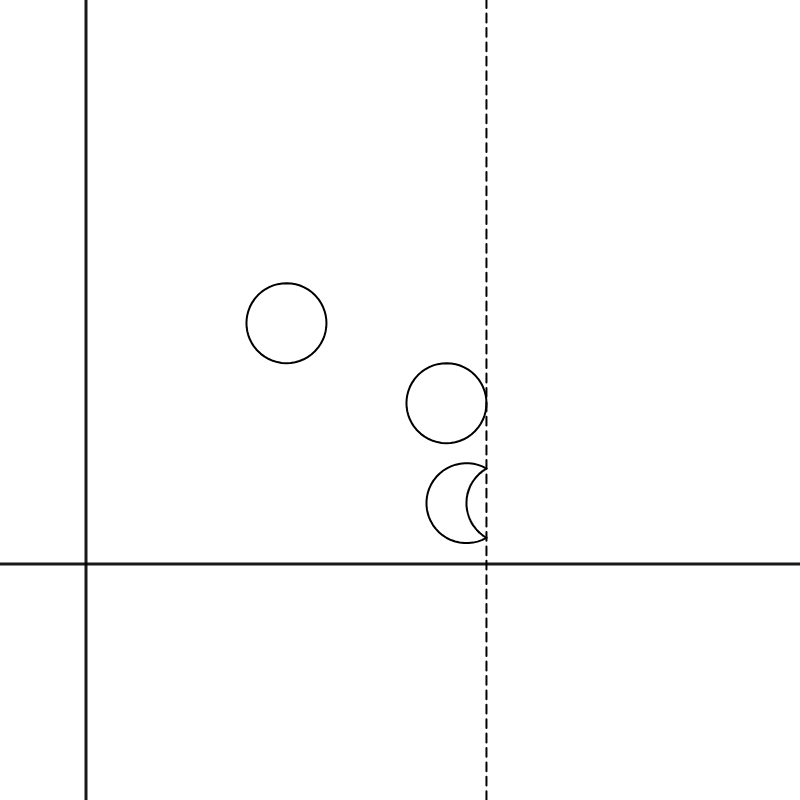
\includegraphics[width=0.4\textwidth]{classical-trajectories-one-wall.png}
    \caption{Three examples of classical trajectories of a particle in a magnetic field with a wall at $x = a$. The two top most trajectory are unaffected by the wall, while the bottom one was partially flipped by the wall.}
    \label{fig:classical_wall}
\end{figure}
\subsection{The quantum case, one wall}
Now let us look at the quantum case. First, we must select a gauge. We saw in the classical case that there is a distinct way of dividing the trajectories by the value of $x_0$. For this reason, it will be wise to select a gauge that will group together the eigenstates with the same $x_0$. That gauge is
\begin{equation}
    A_x = 0 \qquad A_y = Bx \qquad A_z = 0 \rightarrow \boldsymbol{B} = (0, 0, B)
\end{equation}
This results in the Hamiltonian
\begin{equation}
    H_{op} = \frac{\hat{p}_z^2}{2m} + \frac{\hat{p}_x^2}{2m} + \frac{m}{2}\omega_c^2(x - \hat{x}_0)^2 + U(x)
\end{equation}
where
\begin{equation}
    \hat{x}_0 = -\frac{l^2}{\hbar}\hat{p}_y \qquad l = \sqrt{\frac{\hbar}{qB}}
\end{equation}
is an operator corresponding to the classical $x_0$ and contains the remaining degeneracy in the state. The time independent Schrodinger equation $H_op \psi = E\psi$ is then seperable to the three different spatial DOF, and the eigenstates are very easy to find\footnote{Also they are written in the notes}:
\begin{equation}
\label{eq:full-solution-1d}
    \psi(\boldsymbol{r}) = \frac{1}{\sqrt{L_yL_z}}\phi(x) e^{-ix_0y/l^2} e^{ik_zz}
\end{equation}
Where $L_y$ and $L_z$ are very large but finite interval used to create periodic boundary conditiosn on the $y$ and $z$ axes and $\phi(x)$ is a solution to the one dimensional eigenvalue equation
\begin{equation}
\label{eq:one-d-landua}
    \left[
        \frac{\hat{p}_x^2}{2m} + \frac{m}{2}\omega_c^2(x - x_0)^2 + U(x)
    \right]\phi(x) = \varepsilon \phi(x) \qquad \varepsilon = E - \frac{(\hbar k_z)^2}{2m}
\end{equation}
The fact that $U(x > a) = \infty$ means that the wave function must be zero in this segment, giving us the boundary condition
\begin{equation}
\label{eq:one-d-landau-boundary}
    \phi(a) = 0
\end{equation}
While for $x < a$, equation \ref{eq:one-d-landua} is reduced to
\begin{equation}
    \left[
        \frac{\hat{p}_x^2}{2m} + \frac{m}{2}\omega_c^2(x - x_0)^2
    \right]\phi(x) = \varepsilon \phi(x)
\end{equation}
This is a harmonic oscillator, but since it does not span the entire real line, the usual solutions are not applicable here. Instead, we can use the generic before-boundary-conditions solution:
\begin{equation}
    \phi_{\nu,x_0}(x) = A \mathcal{D}_\nu\left(\frac{x - x_0}{l}\right) + B \mathcal{D}_\nu\left(\frac{x_0 - x}{l}\right)
\end{equation}
where $\mathcal{D}_\nu(x)$ are the Parabolic cylinder function\footnote{For further reading and the source of the usage of these functions, see \url{https://dlmf.nist.gov/12}}, which are the solutions to
\begin{equation}
    \left[\frac{d^2}{dx^2} + (a_2x^2 + a_1x + a_0)\right]\mathcal{D}(x) = 0
\end{equation}
Without boundary conditions. Normalizing as $x \rightarrow -\infty$, we get that $B = 0$. Using the boundary condition in equation \ref{eq:one-d-landau-boundary}, we get:
\begin{equation}
    \mathcal{D}_\nu\left(\frac{a - x_0}{l}\right) = 0
\end{equation}
In other words, for the $\phi_{\nu, x_0}$ to solve equation \ref{eq:one-d-landua}, $(a - x_0)/l$ must be a root of $\mathcal{D}_\nu$. Since each Parabolic cylinder function has $\lfloor\nu\rfloor$ distinct roots for odd $\lfloor\nu\rfloor$ and $\lfloor\nu\rfloor + 1$ distinct roots for even $\lfloor\nu\rfloor$, this equation shows the relationship between $\epsilon$, $x_0$, and $\nu$, and thus it gives the energy spectrum. For each $x_0$, the position of the zero relative to the center of the function $a - x_0$ is different. Therefore, for each $x_0$ we get different energy spectrum.
\newline
Let us now look at the different cases. The roots of $\mathcal{D}_\nu$ are distributed as such:
\begin{itemize}
    \item For $\nu < 0$, $\mathcal{D}_\nu$ has no real roots.
    \item For $0 < \nu < 1$, $\mathcal{D}_\nu$ has no positive real roots.
    \item For $\nu = n$ is a positive integer, we get
    \begin{equation}
        \mathcal{D}_n(x) = 2^{-n/2}e^{-x^2/4}\mathcal{H}_n(x)
    \end{equation}
    where $\mathcal{H}_n$ are the Hermite polynomials, well known from the normal solution of the QHO\footnote{Quantum harmonic oscillator}. Since $\mathcal{H}_n$ is an $n$-th degree polynomial, $\mathcal{D}_n$ has $n$ roots.
    \item For $n < \nu < n+1$ for a positive integer $n$, $\mathcal{D}_\nu$ has $n$ positive roots.
\end{itemize}
This allows us to conclude this discussion by expressing the energy spectrum in each $x_0$.
\begin{itemize}
    \item For $x_0$ where $|x_0 - a| \gg l$, the trajectory is very far from the wall and there is no effect of the wall on the energy levels. In this case we get the same energy spectrum as the QHO.
    \item For $x_0$ where $|x_0 - a| \sim l$, the trajectory is close enough to the wall that it would interrupt the energy spectrum, and only the polynoials where equation \ref{eq:one-d-landau-boundary} is satisfied are allowed. In these cases there usually won't be a solution for small values of $\nu$, but using the high-$\nu$ expansion and the continuity of the root as a function of $\nu$, we can conclude that for every $x_0$ there exists some $\nu$ that satisfies equation \ref{eq:one-d-landau-boundary}. We expect then that the energy near the wall will be much higher then the energy far away from it.
    \item For $x_0$ where $|x_0 - a| \ll l$, we can approximate $x_0 \approx a$, and therefore the solutions approach those of the half QHO, meaning only the odd solutions (up to normalization). This range represent a very small area of our parameter space and therefore doesn't contribute much to the overall image. It can be ignored from now on.
    \begin{equation}
        \mathcal{D}_n(x) = 2^{-n/2}e^{-x^2/4}\mathcal{H}_n(x)
    \end{equation}
    where $n = 2k+1$ is odd\footnote{The odd solutions survive because they satisfy $\phi(0) = 0$}.
\end{itemize}
\subsection{Current densities and total currents}
To calcualte the current densities, we use the equation
\begin{equation}
    \boldsymbol{j}(\boldsymbol{r}) = \frac{iq\hbar}{2m}\sum_{spin}\left(\psi\nabla\psi^* - \psi^*\nabla\psi\right) - \frac{q^2}{m}\boldsymbol{A}\sum_{spin}\left(\psi\psi^*\right)
\end{equation}
Assigning equation \ref{eq:full-solution-1d} into this definition, we get:
\begin{equation}
\begin{gathered}
    \boldsymbol{j}(\boldsymbol{r}) = \left[
        \frac{iq\hbar}{2mL_yL_z}\left(
        \left(\phi_{\nu,x_0}'(x), i\frac{x_0}{l^2}, -ik_z\right) - 
        \left(\phi_{\nu,x_0}'(x), -i\frac{x_0}{l^2}, ik_z\right)
    \right) - \frac{q^2}{mL_yL_z}\left(0, Bx, 0\right)
    \right]\phi^2(x) = \\ =
    \frac{q}{L_yL_z}\left(0, \omega_c\left(x - x_0\right), \frac{\hbar k_z}{m}\right)\phi_{\nu,x_0}^2(x)
\end{gathered}
\end{equation}
Where we used $\hbar/l^2 = qB = m\omega_c$. Renaming
\begin{equation}
    \rho_{\nu,x_0} = \frac{1}{L_yL_z}\phi_{\nu,x_0}^2(x)
\end{equation}
we get
% TODO there is a minus error from the last part to here. Find it. This is the correct expression though.
\begin{equation}
    j_x = 0 \qquad j_y = q\omega_c(x-x_0)\rho_{\nu,x_0} \qquad j_z = \frac{\hbar q k_z}{m}\rho_{\nu,x_0}
\end{equation}
The density $\rho_{\nu,x_0}$ is symmetric around $x_0$ only when $\nu$ is an integer. In this case, the current density is antisymmetric and the total current is zero. These solutions, in the range far from the wall $|x_0 - a| \gg l$, are identical to those of the QHO without the wall.
\newline
The closer we get to the wall, the more we go into the high energy area $|x_0 - a| \sim l$. In this area, the density generally doesn't have a defined symmetry, which means the total current density in this area is not zero. This is the edge current, which is a result of a non-uniform energy density along the $x_0$ axis:
\begin{equation}
    I_y(\nu, x_0) = -\frac{q}{m\omega_CL_y}\frac{\partial \epsilon_\nu}{\partial x_0}
\end{equation}

\subsection{The other wall}
Now let us add the other wall at $x = -a$. This gives us a new proper length to the porblem $2a$, and it is worth seperating the porblem into cases by its relation with $l$, the existing proper length in the problem.
\newline
In the first case $2a \gg l$, meaning the two walls bearly interact. Each of them act as its own wall, and the solutions that are close to one wall and are therefore affected by it are far enough from the other wall to not be affected by it.
\newline
The second case $2a \ll l$. In this case, the only solutions that survive are those for which $|x_0 \pm a| \ll l$. With one wall we could approximate that to $x_0 = a$, but this wouldn't work when there are two walls. Instead, we require that both walls are on roots of the wave function
\begin{equation}
    \phi(a) = \phi(-a) = 0
\end{equation}
which means this time $x_0 \approx 0$ instead, and we only take solutions where $\mathcal{H}_n(a/l) = 0$. But such solutions might not exist in the range at all. For instance, $\mathcal{H}_2(x) = 0$ when $x = \pm 0.5$, $\mathcal{H}_3(x) = 0$ when $x = 0, \pm \sqrt{1.5}$, and $\mathcal{H}_4(x) = 0$ when $x = \pm \sqrt{1.5 \pm \sqrt{1.5}}$. Remembering that those solutions are for $x = a/l$, we can see that for them to coincide with the range requirement $2a \ll l$ a very high level of energy is required.
\newline
The last type of solutions is $2a \sim l$, in which both near wall solutions $|x_0 - a| \sim l$ and on wall solutions $|x_0 - a| \ll l$ survive, while the far from wall solutions don't. 
\newline
Both in the far-away case $2a \gg l$ and in the middlerange case $2a \sim l$, the edge currents are similar to those of the previous case and opposite to one another, therefore summing to zero net current. In the small case $2a \ll l$, there are bearly any solutions, and therefore bearly any currents.
\subsection{The $U(y)$ case}
To equivilant case where the well $U(y)$ is described along the $y$ axis can be solved by simply choosing the "opposite" gauge, where $y_0$ contains the degeneracy of the state. In this case, we will write
\begin{equation}
    \boldsymbol{A} = (-By, 0, 0)
\end{equation}
And therefore:
\begin{equation}
    H_{op} = \frac{\hat{p}_z^2}{2m} + \frac{\hat{p}_y^2}{2m} + \frac{m}{2}\omega_c^2(y - \hat{y}_0)^2 + U(y) \qquad \hat{y}_0 = -\frac{l^2}{\hbar}\hat{p}_x
\end{equation}
\begin{equation}
    \psi(\boldsymbol{r}) = \frac{1}{\sqrt{L_yL_z}}\phi(y)e^{-iy_0x/l^2}e^0ik_zz
\end{equation}
Where $\phi(y)$ are again the parabolic cylinder function. This will result in the current densities
\begin{equation}
    j_x = q\omega_c(y-y_0)\rho_{\nu,y_0}
    \qquad
    j_y = 0
    \qquad
    j_z = \frac{\hbar q k_z}{m}\rho_{\nu,y_0}
\end{equation}

\section{Field with root-square dispersion relation}
\subsection{From dispersion relation to field}
Let us look for the field that satisfies the dispersion relation
\begin{equation}
    \epsilon(p) = \sqrt{v^2p^2 + \epsilon_0^2}
\end{equation}
Or, equivilantly
\begin{equation}
    \epsilon^2 = v^2p^2 + \epsilon_0^2
\end{equation}
This can be written in the form of a field equation
\begin{equation}
\label{eq:field-equation-1}
    \frac{\partial^2}{\partial t^2}\phi(x,t) = \left[v^2\frac{\partial^2}{\partial x^2} - \epsilon_0^2\right]\phi(x,t)
\end{equation}
The solutions to which are:
\begin{equation}
    \phi(x,t) = e^{kx \pm \omega t + \alpha}
\end{equation}
Where, of course $\omega = \epsilon/\hbar$ and $k = p/\hbar$. Now, let us find the Hamiltonian for this field equation. Using the difference between the new field equation and the field equation for a linear dispersion relation, let us try the Hamiltonian
\begin{equation}
    H[\pi, \phi] = \int_0^L dx \left[\frac{1}{2}\pi^2 + \frac{v^2}{2}\left(\frac{\partial \phi}{\partial x}\right)^2 + \frac{1}{2}\epsilon_0^2\phi^2\right]
\end{equation}
This Hamiltonian gives:
\begin{equation}
    \frac{\partial \phi}{\partial t} = \pi
    \qquad
    \frac{\partial \pi}{\partial t} = v^2 \frac{\partial^2 \phi}{\partial x^2} - \epsilon_0^2 \phi
\end{equation}
Which combine exactly to give equation \ref{eq:field-equation-1}, meaning this Hamiltonian describes our dispersion relation. Now let us find the mechanical momentum. The mechanical momentum is by definition conserved, and its continuity equation connected between the time derivative of its density and the space derivative of the Hamiltonian density:
\begin{equation}
    \frac{\partial \mathcal{P}}{\partial t} = -\frac{\partial \mathcal{H}}{\partial x}
\end{equation}
Using our Hamiltonian, the Hamiltonian density is
\begin{equation}
    \mathcal{H} = \frac{1}{2}\pi^2 + \frac{v^2}{2}\left(\frac{\partial \phi}{\partial x}\right)^2 + \frac{1}{2}\epsilon_0^2\phi^2
\end{equation}
And so the mechanical momentum density is still
\begin{equation}
    \mathcal{P} = -\pi\frac{\partial \phi}{\partial x}
\end{equation}
This work since
\begin{equation}
    \frac{\partial \mathcal{P}}{\partial t} = -\frac{\partial \pi}{\partial t}\frac{\partial \phi}{\partial x} - \pi\frac{\partial^2 \phi}{\partial x \partial t} = -\left(v^2 \frac{\partial^2 \phi}{\partial x^2} - \epsilon_0^2 \phi\right)\frac{\partial \phi}{\partial x} - \pi\frac{\partial \pi}{\partial x} = -\frac{\partial}{\partial x} \left[
        \frac{1}{2}\pi^2 + \frac{v^2}{2} \left(\frac{\partial \phi}{\partial x}\right)^2 + \frac{1}{2}\epsilon_0^2\phi^2
    \right] =  -\frac{\partial \mathcal{H}}{\partial x}
\end{equation}
And so the mechanical momentum is still
\begin{equation}
    \mathbb{P} = -\int_0^L \pi\frac{\partial \phi}{\partial x} dx
\end{equation}
\subsection{The different terms in the field equation}
The field equations has three terms: the second time derivative, the second space derivative, and the new addition $\epsilon_0^2$. Without $\epsilon_0^2$, the equation is identical to the equation we saw in class. The two remaining terms are responsible for the propagation of the wave along the string. Since in that case the second derivative with respect to time equals the second derivative with respect to $x$, every motion of the field in any position must relate to a motion of the field in positions next to it, causing the motion to propagate along the string.
\newline
The new term reduces this coupling by the fact that every motion in the field is now divided between the term related to the field and the term related to its space derivative. This means that every motion in the field at any position is now reduced by a term related to the field and then passed on to the positions next to it. This makes the new term into a mass term, delaying the motion and slowing it down.
\subsection{The quantum mechanical description of a free motion}
Similar to the massless field, we can look at the field as a collection of independent quanta. These quanta move with their phase velocity
\begin{eqnarray}
    v_\phi = \frac{\epsilon}{p} = \sqrt{v^2 + \left(\frac{\epsilon_0}{p}\right)^2}
\end{eqnarray}
The wave packets of these quanta move with the group velocity:
\begin{equation}
    v_g = \frac{\partial \epsilon}{\partial p} = \frac{v^2p}{\sqrt{v^2p^2 + \epsilon_0^2}}
\end{equation}
It can be seen that the higher the mass, the slower the wave packet is. This is a direct result of the mass being the source of dispersion in these equations and the slowing factor for the propagation of the motion.
\subsection{Three dimensions}
The extension to three dimensions is trivial. First, the field equation becomes
\begin{equation}
    \frac{\partial^2}{\partial t^2}\phi(x,t) = \left[v^2\nabla^2 - \epsilon_0^2\right]\phi(x,t)
\end{equation}
Which means that Hamiltonian is
\begin{equation}
    H[\pi, \phi] = \int_0^L dx \left[\frac{1}{2}\pi^2 + \frac{v^2}{2}\left(\nabla \phi\right)^2 + \frac{1}{2}\epsilon_0^2\phi^2\right]
\end{equation}
and the mechanical momentum is
\begin{equation}
    \mathbb{P} = -\int_V \pi(\nabla\phi) dr
\end{equation}
and the above phase and group velocity are identical to those of one dimension, just in each of the three dimensions.

\section{Striked string}
The string is "striked" at time $t = 0$ which gives us the starting configuration $\phi_0(x) = \phi(x,0)$. Classically, the way to solve this is to transform the starting configuration to the normal modes representation, and then propagate each of them in time. Assuming, as we did in class, that the string has periodic boundary conditions and can therefore contain traveling waves, we can find $Q_k$ and $P_k$ using
\begin{equation}
\begin{gathered}
    Q_k = \frac{1}{\sqrt{L}}\int_0^L dx \left[\phi_0(x)\sin(kx) - \frac{1}{\omega_k}\pi_0(x)\cos(kx)\right]
    \\
    P_k = \frac{1}{\sqrt{L}}\int_0^L dx \left[\pi_0(x)\sin(kx) + \omega_k\phi_0(x)\cos(kx)\right]
\end{gathered}
\end{equation}
This, of course, requires to know $\pi_0(x)$. If the guitar string is "struck", let us assume that $\pi_0(x) = 0$, and so:
\begin{equation}
\begin{gathered}
    Q_k(0) = \frac{1}{\sqrt{L}}\int_0^L \phi_0(x)\sin(kx) dx
    \\
    P_k(0) = \frac{1}{\sqrt{L}}\int_0^L \omega_k\phi_0(x)\cos(kx) dx
\end{gathered}
\end{equation}
In which case
\begin{equation}
    \phi(x,t) = \frac{1}{\sqrt{L}}\sum_k \left[Q_k(t)\sin(kx) + \frac{1}{\omega_k}P_k(t)\cos(kx)\right]
\end{equation}
Where
\begin{equation}
\begin{gathered}
    Q_k(t) = Q_k(0)\cos(\omega_k t) + \frac{1}{\omega_k}P_k(0)\sin(\omega_k t)
    \\
    P_k(t) = -\omega_k Q_k(0)\sin(\omega_k t) + \frac{1}{\omega_k}P_k(0)\cos(\omega_k t)
\end{gathered}
\end{equation}
The change in the quantum mechanical case is trivial. The transformation to the normal modes representation remains the same, and we get the same dynamical picture. The key difference is that we cannot think about a starting configuration of the entire field, since this cannot be measured (it is impossible to renormalize all normal modes at the same measurement). This means we have to understand the starting configuration as the peak of the probability function.
\end{document}